\documentclass[aspectratio=169]{beamer}
\usetheme{einfra2}

\usepackage[utf8]{inputenc}
\usepackage[czech]{babel}

\title{Predikce hmotnostního spektra neuronovými sítěmi}
\author{Filip Jozefov, Adam Hájek, Aleš~Křenek}
\date{Sitsem, 14.9.2023, Telč}

\begin{document}
\makeatletter
\maketitle

\begin{frame}
{Cesta tam}{\dots a ještě ne zpátky}

\begin{itemize}
\item Známe vzorec molekuly, zpravidla jako tzv.\ SMILES: \qquad
\vbox to0pt{
\hsize=1em

\includegraphics[height=12ex]{thc-formula}
\par
\vss
}

\medskip
CCCCCc1cc(c2c(c1)OC([C@H]3[C@H]2C=C(CC3)C)(C)C)O 


\medskip
\pause
\item Chceme predikovat hmotnostní spektrum této látky 

\medskip
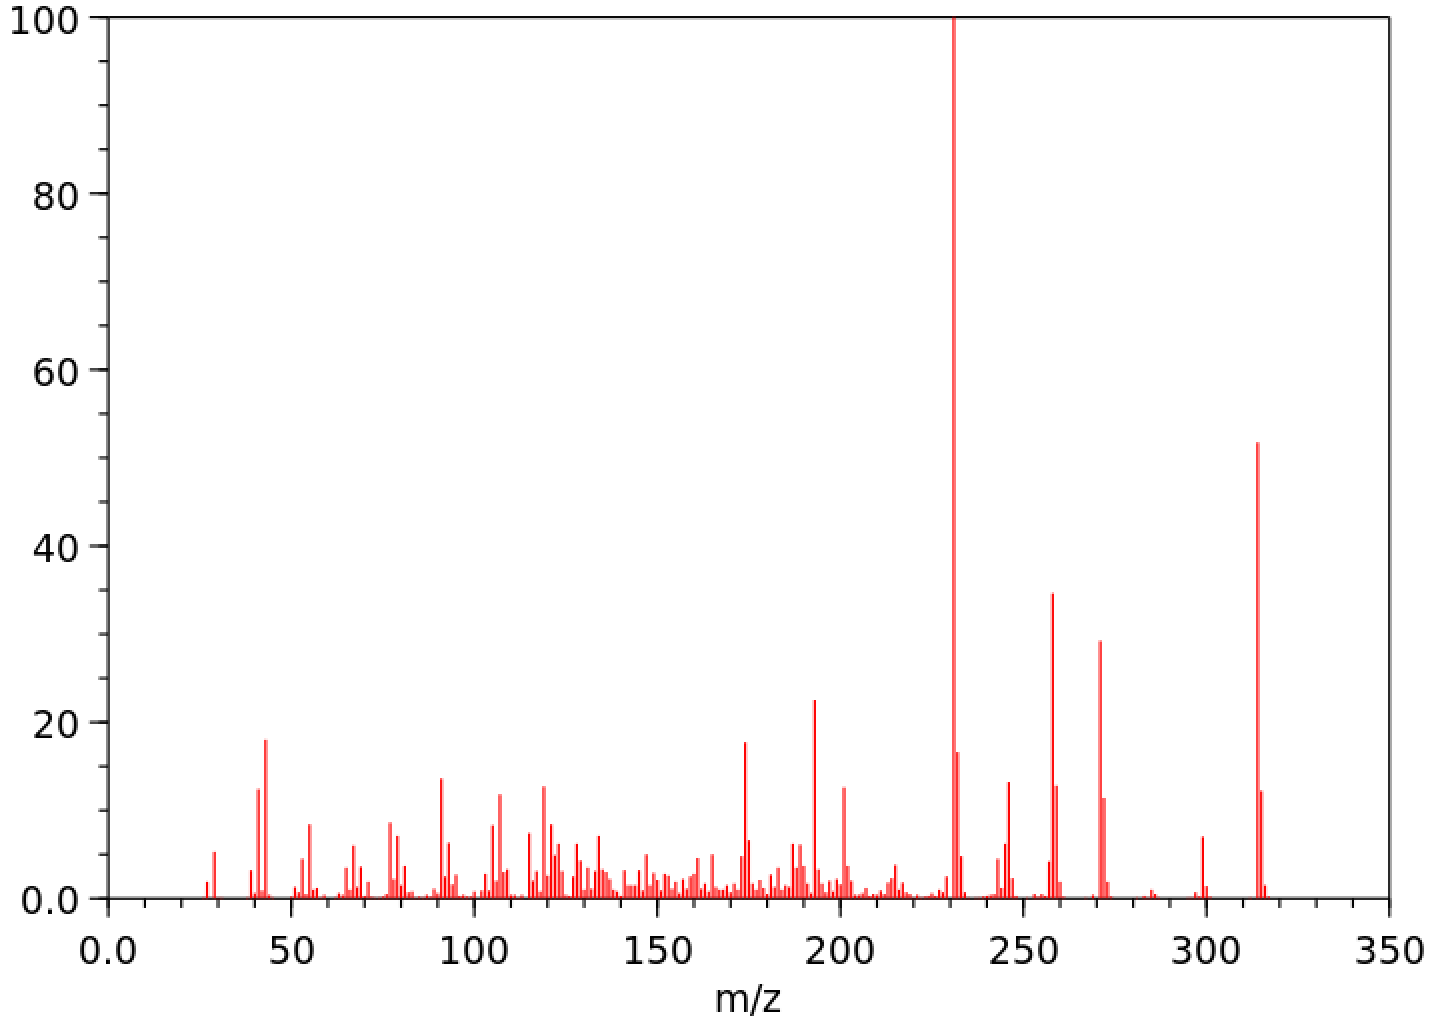
\includegraphics[width=.4\hsize]{thc-spec}
\end{itemize}
\end{frame}

\begin{frame}
{Možné přístupy}
\begin{itemize}
\item \emph{Ab initio} -- kvantově-chemická simulace dějů při štěpení molekuly
\begin{itemize}
\item potenciálně nejpřesnější
\item výpočetní náročností neúnosné (dny až týdny výpočtu pro jednu molekulu)
\end{itemize}
\medskip
\item Empirické -- založené na expertních pravidlech štěpení vazeb atd.
\begin{itemize}
\item neopřesné, omezená doména
\end{itemize}
\medskip
\item \textbf{Strojové učení} na základě desítek až stovek tisíc příkladů
\begin{itemize}
\item uspokojivá rychlost i přesnost, ale stále je co dělat
\item neuronové sítě, inspirace jazykovými modely
\end{itemize}
\end{itemize}
\end{frame}

\begin{frame}
{NEIMS}{\dots jednodušší už to být nemůže}
\begin{itemize}
\item Neural Electron-Ionization Mass Spectrometry
\begin{itemize}
\item J.~N.~Wei et.~al, 2019, \url{http://doi.org/10.1021/acscentsci.9b00085}
\end{itemize}
\pause
\medskip
\item Molekula popsána systémem \emph{fingerprintu}
\begin{itemize}
\item konkrétně délky 4096 bitů, ,,1`` znamená výskyt specifické podstruktury
\item standardizovaný postup výpočtu
\end{itemize}
\item Spektrum kódováno přímočaře jako vektor
\begin{itemize}
\item jedna složka pro každou celočíselnou hodnotu $m/z$
\end{itemize}
\end{itemize}
\end{frame}

\begin{frame}
{NEIMS}
\begin{itemize}
\item Jednoduchá architektura neuronové sítě
\begin{itemize}
\item MLP, 7 skrytých vrstev po 2000 neuronech
\item ReLU, dropout 25\,\%
\end{itemize}
\item Zdvojená poslední vrstva
\begin{itemize}
\item fingerprinty vystihují lépe malé fragmenty, model je přesnější pro malá $m/z$
\item přidána tzv. \emph{reverzní predikce}, počítá špičky $M-m/z$ z~téže předposlední vrstvy
\end{itemize}
\end{itemize}
\end{frame}

\begin{frame}
{NEIMS}
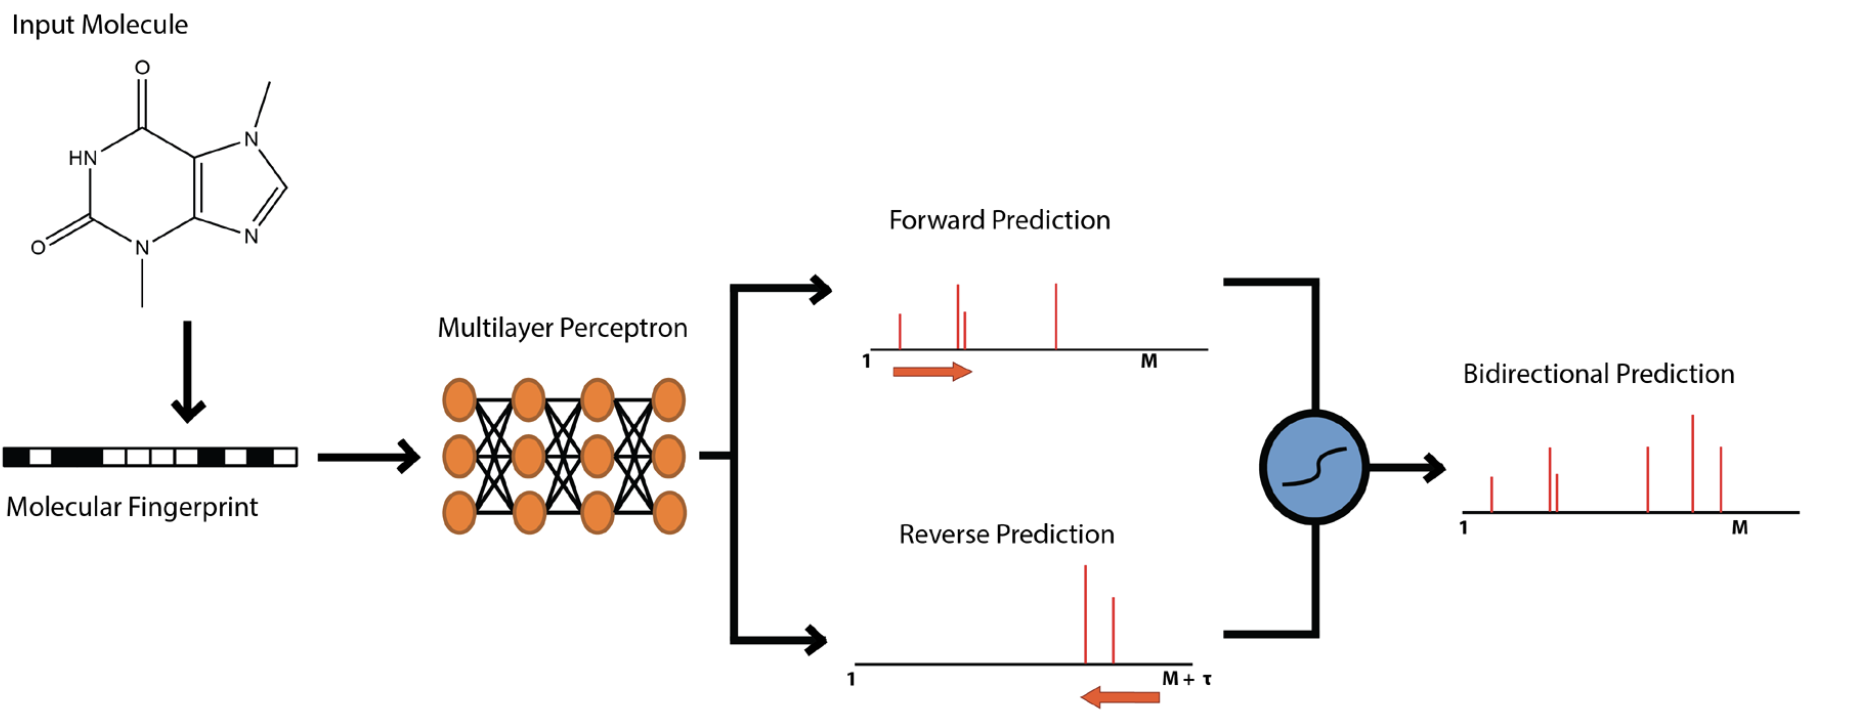
\includegraphics[width=\hsize]{neims.png}
\end{frame}

\begin{frame}
{NEIMS -- výsledky}
\begin{itemize}
\item Společná trénovací (113k) a testovací (28k) sada pro všechny modely 
\item $\textbf{DP} = 0.832\pm0.108, \textbf{SDP}=0.828\pm 0.136$ na testovací sadě
\item Dobré, nikoli vynikající, rychlý tréning i inference
\end{itemize}
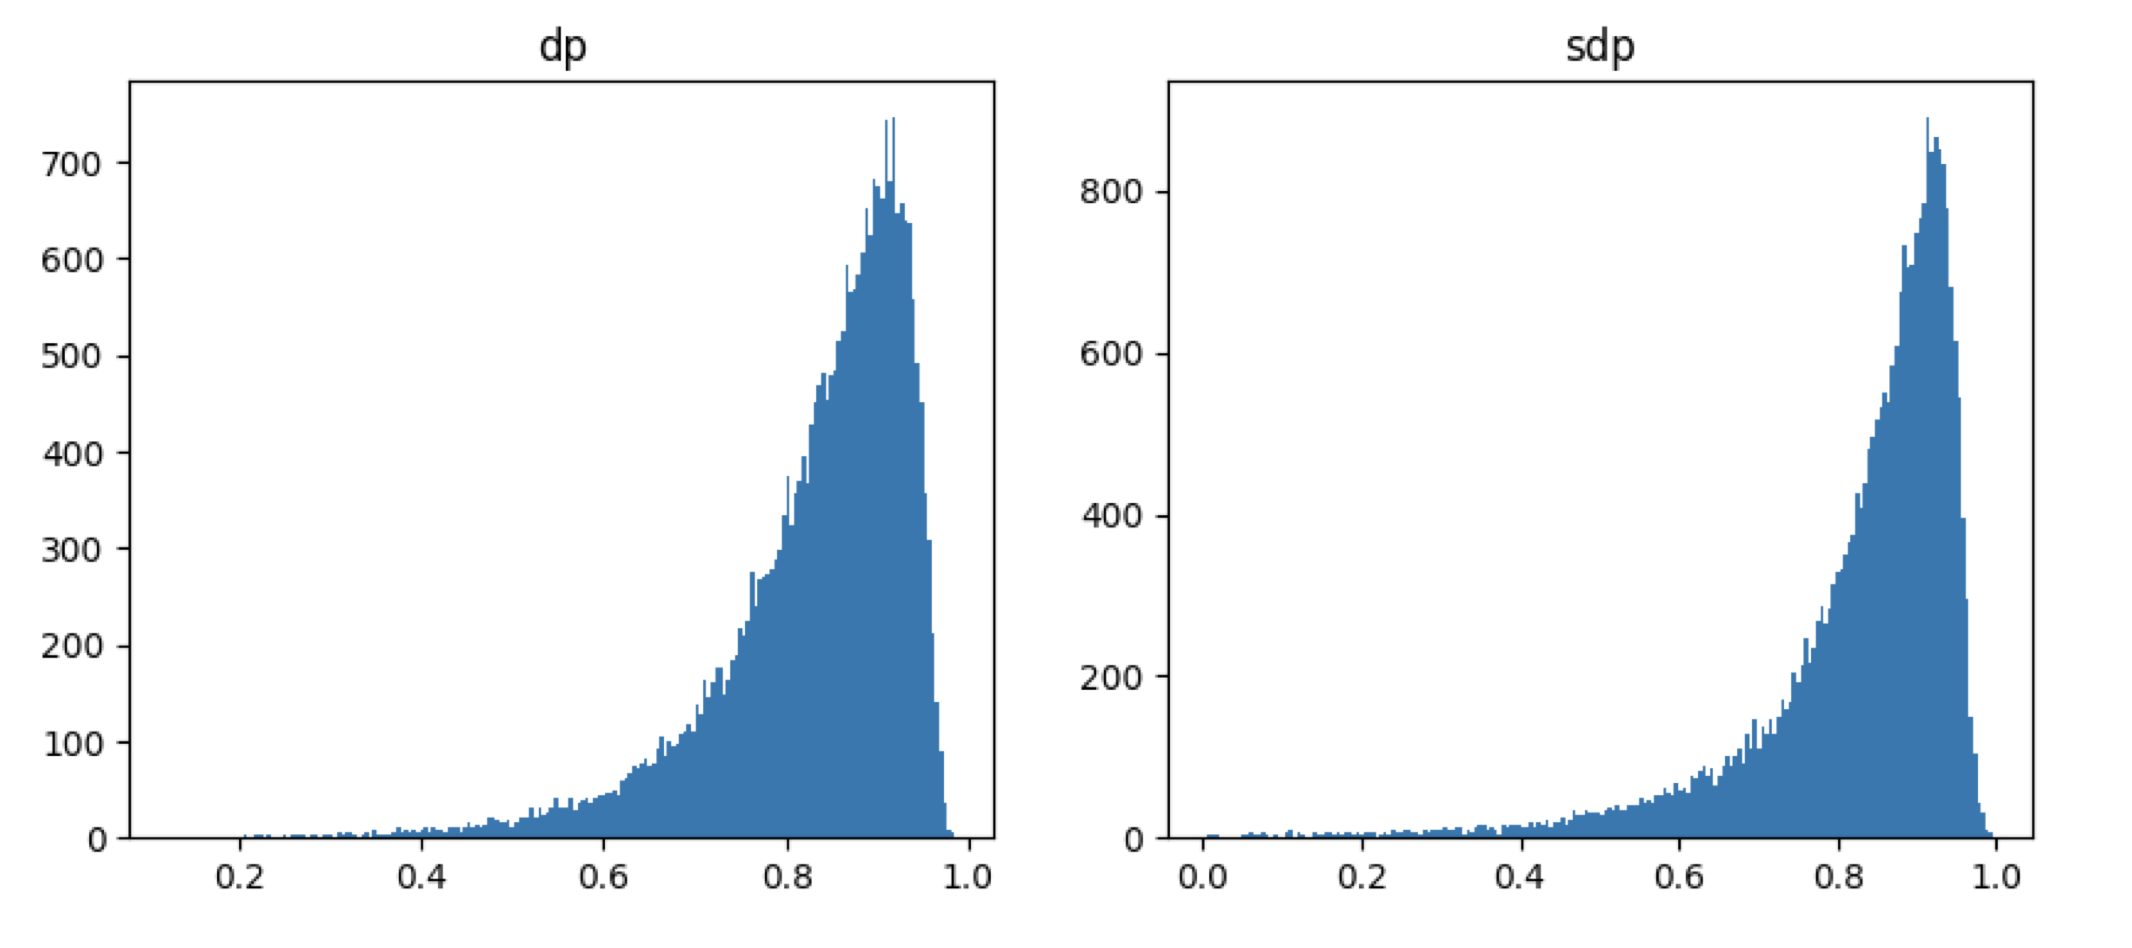
\includegraphics[width=.8\hsize]{neims-hist}

\end{frame}

%Rapid Approximate Subset-Based Spectra Prediction for Electron Ionization–Mass Spectrometry
%Richard Licheng Zhu and Eric Jonas
%Analytical Chemistry 2023 95 (5), 2653-2663
%DOI: 10.1021/acs.analchem.2c02093


\end{document}
